\chapter{Empirical study and results}
\label{cpt:result}
\section{Stock market description}
There are totally 261 trading days in 2016 of US stock market, this thesis selects 1,418 stocks of listing US companies that were traded in all trading days in 2016. Table~\ref{tab:industrytable} shows the titles of 55 industrial sectors corresponding to the summary level of BEA industry codes as well as the number of stocks in each of them.
\begin{longtable}{c|c} 
	\centering
	\textbf{Industrial Sector Title} & \textbf{Stock Count}  \\ \hline
	Computer and electronic products & 326 \\
	Banks, credit intermediation, and related activities&271 \\ 
	Chemical products &241 \\ 
	Funds, trusts, and other financial vehicles	&166\\
	Insurance carriers and related activities&122 \\
	Fabricated metal products	&85 \\
	Utilities&	83 \\
	Food and beverage and tobacco products	&81 \\
	Oil and gas extraction	&77 \\
	Broadcasting and telecommunications	&69 \\
	Machinery&	59 \\
	Computer systems design and related services&	54 \\
	Other retail & 51  \\
	Securities, commodity contracts, and investments & 50 \\
	Wholesale trade & 48 \\
	Miscellaneous professional, scientific, and technical services & 45 \\
	Motor vehicles, bodies and trailers, and parts & 43 \\
	Performing arts, spectator sports, museums, and related activities & 40 \\
	Data processing, internet publishing, and other information services & 35 \\
	Construction & 34 \\
	Support activities for mining & 28 \\
	Petroleum and coal products & 26 \\
	Paper products & 24 \\
	Rental and leasing services and lessors of intangible assets & 22 \\
	Air transportation & 20 \\
	Ambulatory health care services & 20 \\
	Accommodation & 19 \\
	Administrative and support services & 16 \\
	Publishing industries, except internet (includes software) & 16 \\
	Water transportation & 14 \\
	Truck transportation & 14 \\
	Transit and ground passenger transportation & 14 \\
	Plastics and rubber products & 12 \\
	Other transportation and support activities & 11 \\
	Other transportation equipment & 10 \\
	Miscellaneous manufacturing & 10 \\
	Other real estate & 9 \\
	Textile mills and textile product mills & 9 \\
	Furniture and related products & 7 \\
	Electrical equipment, appliances, and components & 7 \\
	Primary metals & 7 \\
	Nonmetallic mineral products & 6 \\
	Hospitals & 6 \\
	Waste management and remediation services & 5 \\
	Rail transportation & 5 \\
	Pipeline transportation & 5 \\
	Motion picture and sound recording industries & 4 \\
	Apparel and leather and allied products & 3 \\
	Nursing and residential care facilities & 3 \\
	Wood products & 3 \\
	Printing and related support activities & 3 \\
	Mining, except oil and gas & 3 \\
	Legal services & 1 \\
	Social assistance & 1 \\
	Other services, except government & 1 \\
	\textbf{Total} & \textbf{2344} \\
	\caption{Part of counts for US stocks by industry \cite{secwebsite}}
	\label{tab:industrytable}
\end{longtable}

It is not hard to see the composition of stock market are mainly dominated by the financial related industry ("Banks, credit intermediation, and related activities", "Funds, trusts, and other financial vehicles", "Insurance carriers and related activities", "Securities, commodity contracts, and investments", etc.) and computer related industry ("Computer and electronic products", "Computer systems design and related services", "Data processing, internet publishing, and other information services", "Electrical equipment, appliances, and components", etc.).

\section{Network construction}
This paper first calculated normalised direct requirement and normalised direct demand values for every sectors using formula~\ref{equ:eio_i} and formula~\ref{equ:eio_o} and cross-correlation coefficients between every stock pairs using formula~\ref{equ:corr}.

According to the figure~\ref{fig:eio_transaction_density}, the transaction densities decrease as threshold of normalised direct requirement and normalised direct demand increase, and their patterns are exactly similar with the same inflection point at around $threshold=0.136$ where the densities begin to decline. Therefore, the values of thresholds for normalised direct requirement and normalised direct demand are set to be equal, i.e., $\theta_{EIO}=\theta_{DD}=\theta_{DR}$,  to filter the directed edges among the stock network.

\begin{figure}
	\begin{center}
		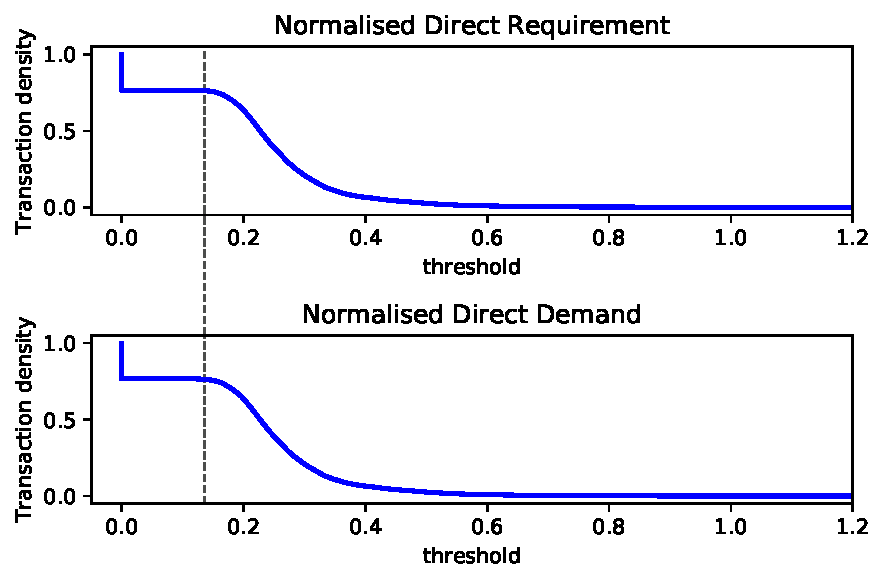
\includegraphics[width=14cm]{eio_transaction_density}
	\end{center}
	\caption{Transaction densities}
	\label{fig:eio_transaction_density}
\end{figure}

\begin{figure}
	\begin{center}
		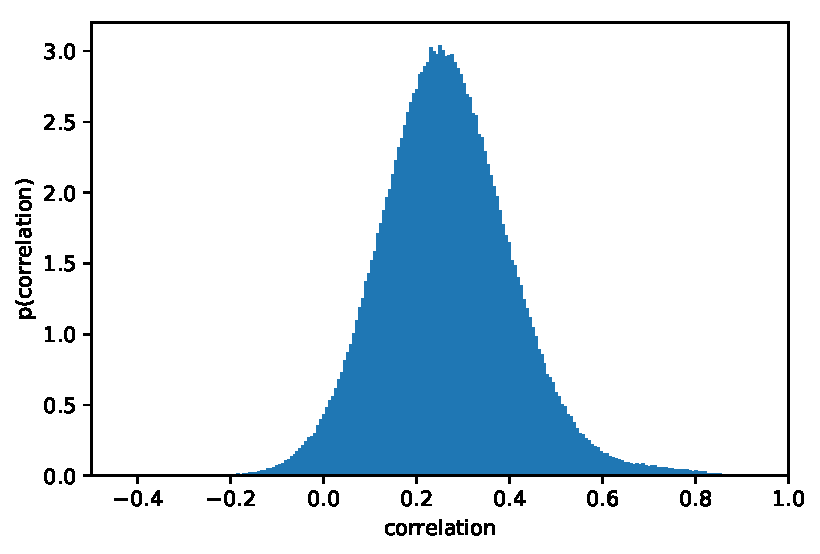
\includegraphics[width=14cm]{correlation_distribution}
	\end{center}
	\caption{Stock price return correlation coefficient distribution}
	\label{fig:correlation_distribution}  
\end{figure}

\begin{figure}
	\begin{center}
		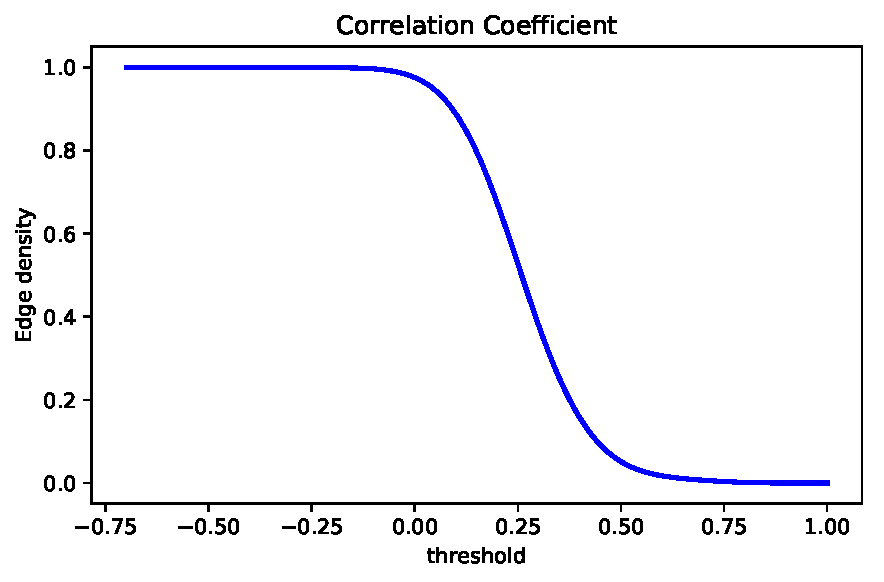
\includegraphics[width=14cm]{correlation_edge_density}
	\end{center}
	\caption{}
	\label{fig:correlation_edge_density}  
\end{figure}

Figure~\ref{fig:correlation_distribution} shows the distribution of stock price correlation coefficients has a shape complies to the normal distribution with long tails. The correlation coefficients are vary from -0.687 to 0.977 with the mean of 0.265. It implies that the prices of most stocks traded in NYSE and NASDAQ usually fluctuate to the same direction, but the patterns are less similar.

% 拟合正态分布或t分布

\begin{figure}
	\begin{center}
		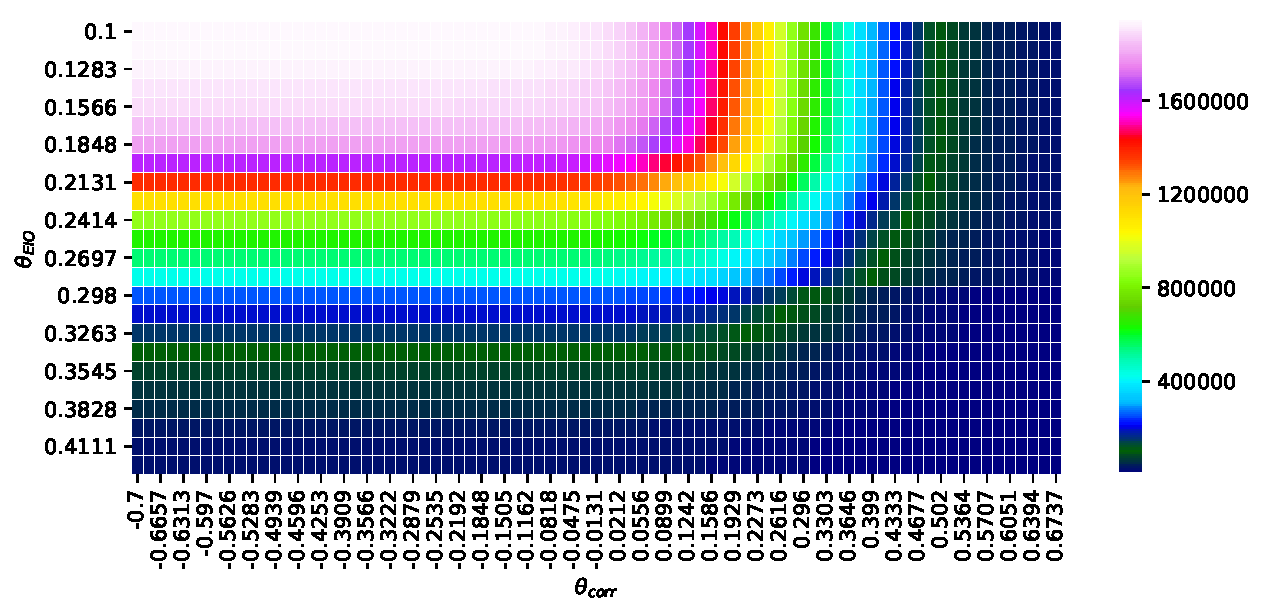
\includegraphics[width=15cm]{amounts_of_edges_threshold}
	\end{center}
	\caption{Numbers of directed edges per EIO-threshold and correlation-coefficient-threshold}
	\label{fig:amounts_of_edges_threshold}  
\end{figure}

Figure~\ref{fig:amounts_of_edges_threshold} shows the number of directed edges remain at the conditions of different value combinations of $\{\theta_{EIO}$, $\theta_{corr}\}$. When both of the thresholds set to be minimal at their own value range, i.e., $\theta_{EIO}=0$ and $\theta_{corr}=-1$, the number of directed edges is $N\times(N-1)=2,009,306$, while $N$ indicates the total number of nodes, which is $1418$. According to the figure~\ref{fig:amounts_of_edges_threshold}, the number of edges will be less than $100,000$, in which case the network has a density of lower than $5\%$, if $\theta_{EIO}\geq0.3545$ or $\theta_{corr}\geq0.5020$. 

\begin{figure}
	\begin{center}
		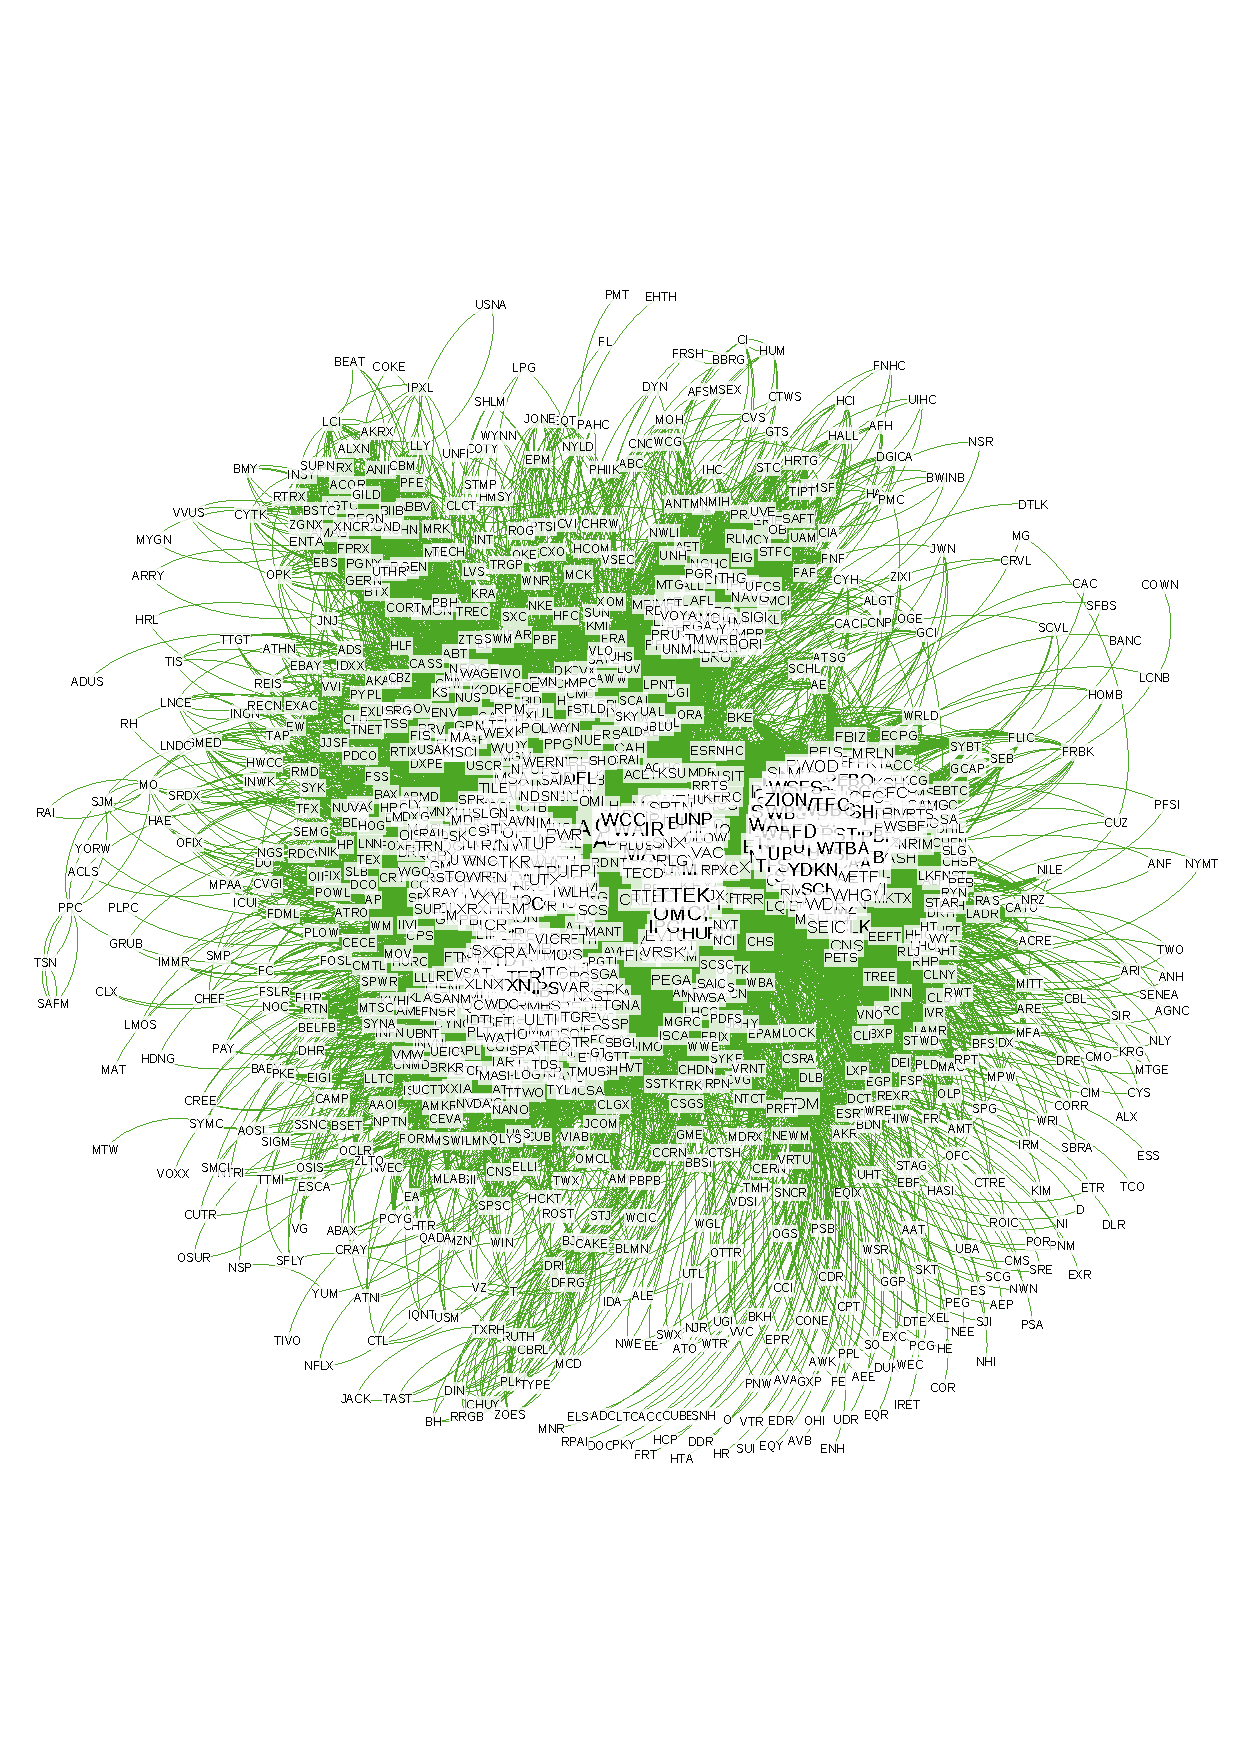
\includegraphics[width=14cm]{Graph_01}
	\end{center}
	\caption{Transaction densities}
	\label{fig:Graph_01}
\end{figure}


It is obvious that the larger values assigned to $\theta_{EIO}$ and $\theta_{corr}$, the more significant will be for the weights and directions of the remaining edges. But if the network becomes too sparse, it can not be strongly or even weakly connected and there would be many independent cliques, hence the network becomes too inefficient to be a senseful network. As a result, this paper selects the threshold-value-pair $\{\theta_{EIO}=0.292, \theta_{corr}=0.379\}$ to construct a directed unweighted network and a directed weighted network for the 2016 US stock market.

%这里放Gephi的图片 可以随机选择一半的结点作为生成

\section{Analysis of the directed unweighted network}
% 对幂指数分布的统计检验
A directed Watts Strogatz small-world (WS) network and a random network with the same number of nodes and similar number of edges with the stock directed unweighted network are generated. Table~\ref{tab:three} compares the main topologies of the three networks.

\begin{table}
	\begin{center}
		\begin{tabular}{|r|c|c|c|}\hline\hline
			Directed networks&Stock network&Small-world network&Random network\\\hline
			Number of nodes&1418&1418&1418\\
			Number of edges&102051&102088&102097\\
			Out-degree distribution&Power-law&Normal&Normal\\
			Average out-degrees&143.94&143.99&144.00\\
			Average path length&2.775&2.005&1.973\\
			Clustering coefficient&0.4675&0.1367&0.05105\\
			Global efficiency&0.2563&0.5161&0.5216\\
			Local efficiency&0.6276&0.5027&0.4456\\
			Assortativity&0.02004&-0.002180&0.001452\\
			\hline\hline
		\end{tabular}
	\end{center}
	\caption{Main properties of stock network, small-world network, and random network}\label{tab:three}
\end{table}

\subsection{Power-law distribution}

According to the table~\ref{tab:three}, the values of average out-degrees of stock network, small-world network and random network are almost the same due to the identical numbers of nodes and edges, but in terms of the distributions of out-degrees, stock network is totally different from the others. 

Figure~\ref{fig:distributionsm} and \ref{fig:distributionrd} show clearly that the out-degree distributions of small-world network and random network follow the normal distribution, i.e, most degree numbers of nodes fall in the middle range, while figure~\ref{fig:G_out_degree_distribution_square} illustrates that for the stock network, only a few number of nodes show higher out-degree, while most nodes are in the positions of low out-degree level. The distribution of the directed stock price return networks follows power-law distribution with the exponent of 4.057.

%Power-law distribution reveals that most of the nodes have a small degree while a few modes have a higher degree.
\subsection{Small-world property}
The average path length of small-world network and random network are both close to 2, indicates that taking any node in the network, it can expect to reach any other nodes just through one node as medium. For stock network, the expectation number of medium nodes is 1.775, which is also a small number for connection, so like small-world and random networks, stock network also has the small-world property.

% Efficiency.

Although the assortativity values for the three networks are all non-significant, 

\subsection{Community structure of the directed unweighted stock network}
The larger value of clustering coefficient for stock network than the other two networks indicating that the nodes in stock network tend to cluster together. Therefore, communities of stock network will be identified implementing the \textit{algorithm~\ref{alg:communitydetection}} for directed networks in this section. According to the composition of industrial sectors of each community, as figure~\ref{fig:community_sector_stacked} shows, the following five communities are identified: (1) Production (2) Finance (3) Livelihood (4) Insurance and chemical products (5) Utilities and financial vehicles.

The communities of production (purple) and livelihood (blue) are sparsely distributed while there are some large-sized nodes acting as hubs of the overall network. The hubs not only connect to the nodes of same communities, but also the externals. These two communities are partially intertwined due to the high relevancy of production industry and livelihood industry. 

Unlike the above two communities, it can be seen from figure~\ref{fig:community_graph} that the community of finance (green) is decentralised, i.e., there is no obvious hubs and the degrees of each node distribute evenly. It also has a very dense structure, connected closely inside and completely exclusive from other nodes or communities. This means the co-movements among financial stocks are incredibly strong and economically they rely tightly to each other.

The other two communities are more interesting because of their peculiar structural features. Every industrial sectors of individual stocks in community are identified to investigate the properties of the community of insurance and chemical products (yellow). As figure~\ref{fig:community_4} illustrates and through the investigation, almost all firms in the upper and lower clusters are in the sectors of "chemical products" and "insurance carriers and related activities" respectively, while firms between the two big clusters, like "MCK" (McKesson) and "CAH" (Cardinal Health), are large medical supplier, pharmaceutical and heathcare service companies with high out-degrees to both of the two clusters. Apart from that, there are also a considerable number of links from the nodes in upper cluster to the hubs of chemical companies. Thus, it is reasonable to infer that the prices of medicines have significant influence to medical insurance industry, additionally the purchases of chemical products of pharmaceutical firms and the sales of chemical products have made pharmaceutical and chemical companies influence to each other.

Another investigation towards the community of utilities and financial vehicles (orange) is conducted by the same measure. As figure~\ref{fig:community_5} illustrates, there is only one huge hub (PDM) which is the company "Piedmont Office Realty Trust" among the whole community while all the others are one-degree nodes located remotely. There are more links from the hub to the rest than the opposite direction, and also the weights of the former links are generally higher. The hub, "Piedmont Office Realty Trust", is a real estate investment trust company, and the rest in the community contains 59 "funds, trusts, and other financial vehicles" firms and 44 "utilities" firms. For a big realty trust enterprise, demand for financial trust business is extremely high, and its successes of investments upon real estates will promote the development of utilities companies. It depicts that the major realty trust enterprise alone has significant influence to all of these financial trust and utilities companies.

\begin{figure}
	\begin{center}
		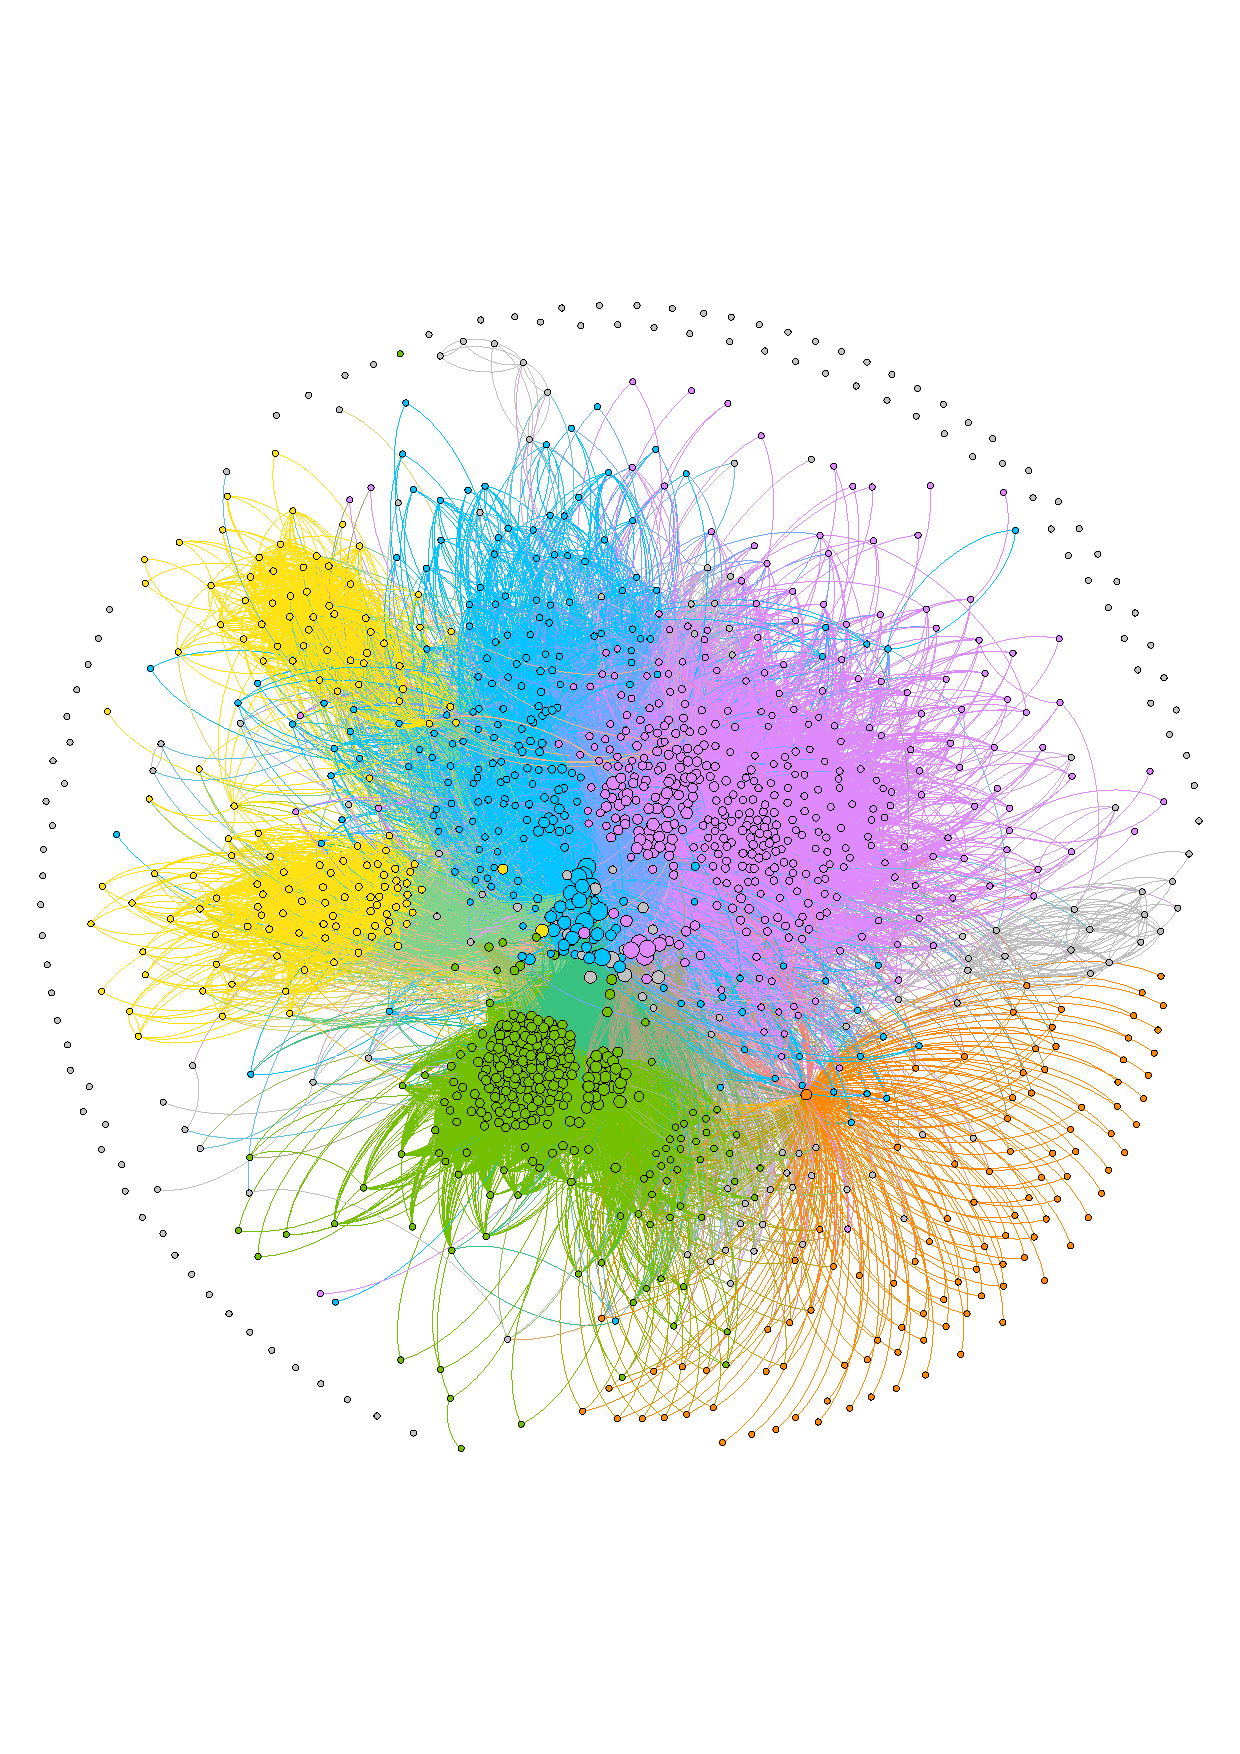
\includegraphics[width=14cm]{community_graph}
	\end{center}
	\caption{Community structure of the 2016 US stock price return network. Five distinct communities are detected represented by different colours of nodes. The direction of edge is  clockwise. The size of nodes and thickness of edges are related to the value of degrees and weights. The grey nodes do not belong to any communities and most of them have zero degree.}
	\label{fig:community_graph}
\end{figure}

\begin{figure} % 各个单独的群落
	\subfloat[Production]{%
		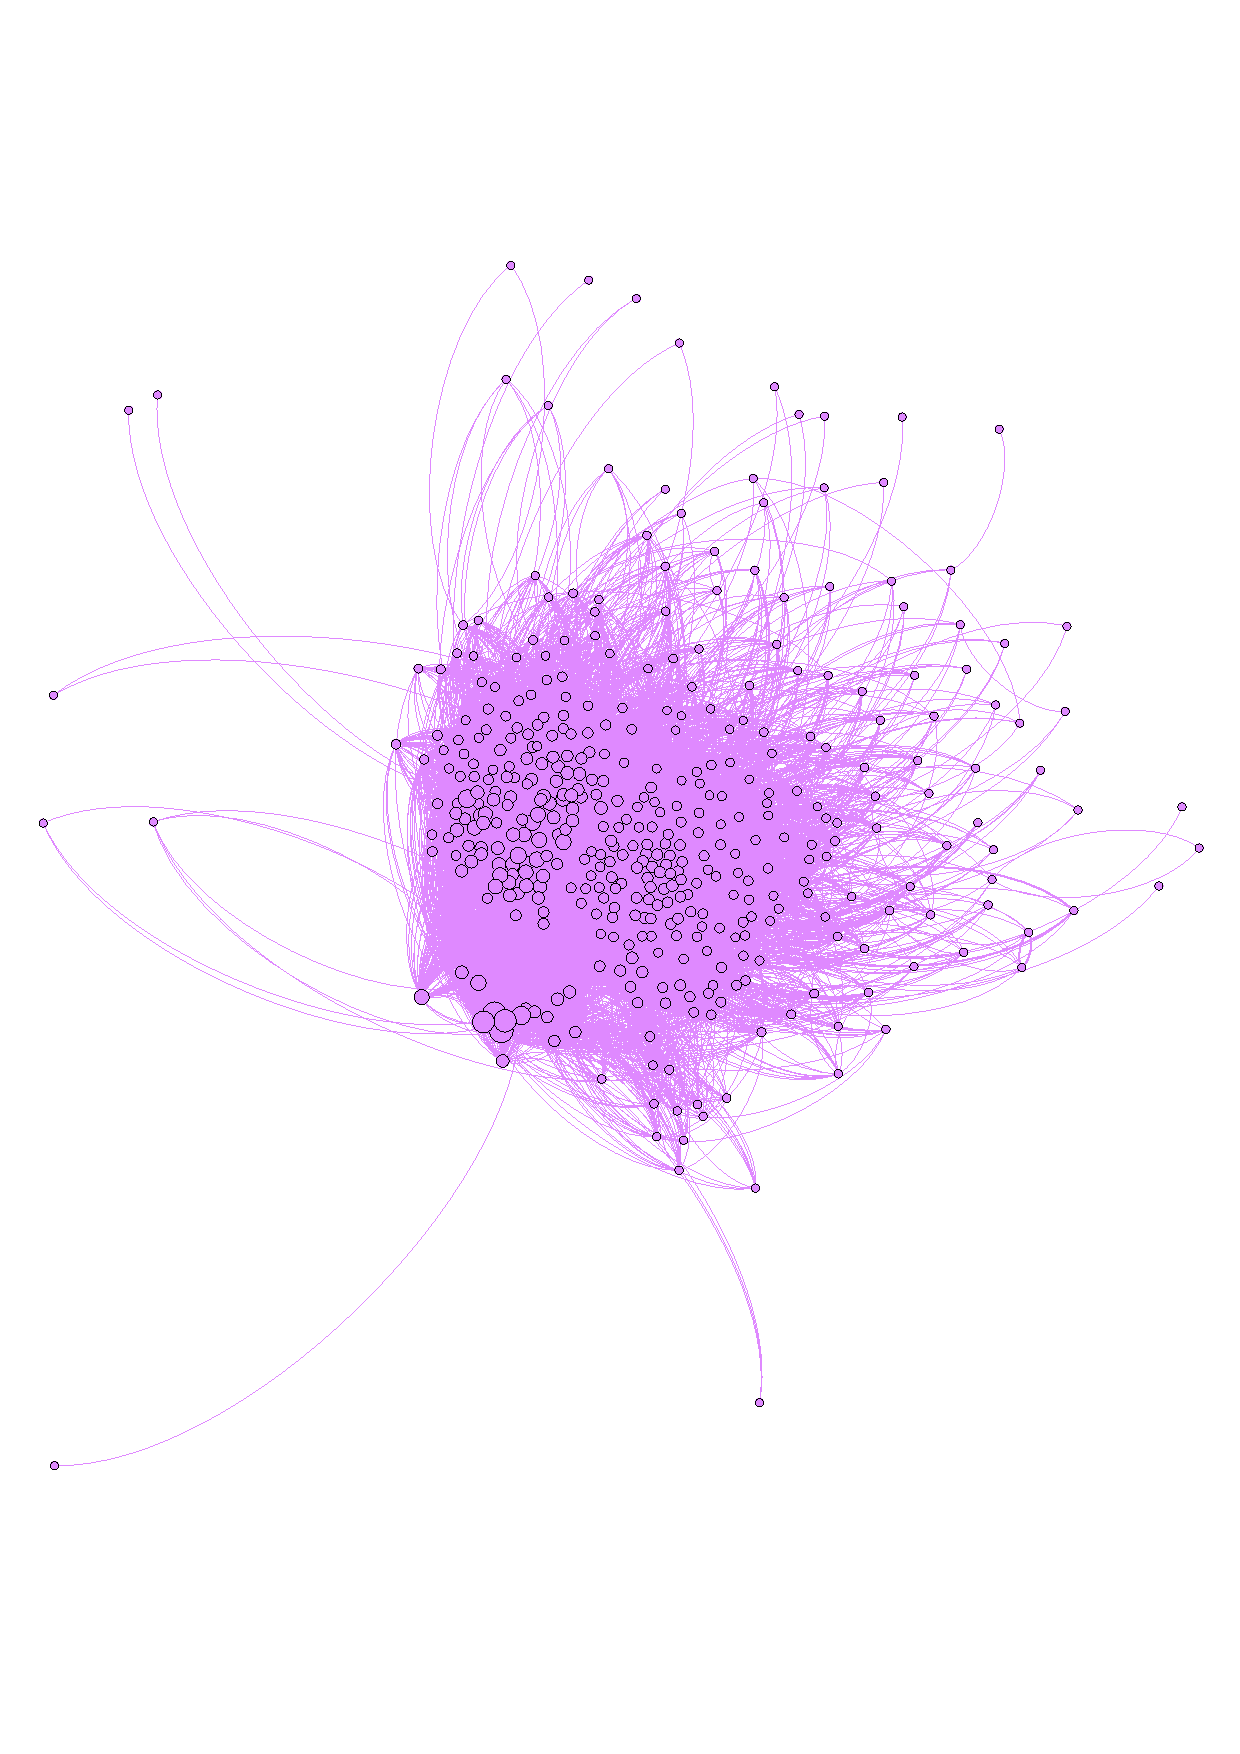
\includegraphics[width=0.45\textwidth]{community_1}%
		\label{fig:community_1}%
	}%
	\hfill%
	\subfloat[Finance]{%
		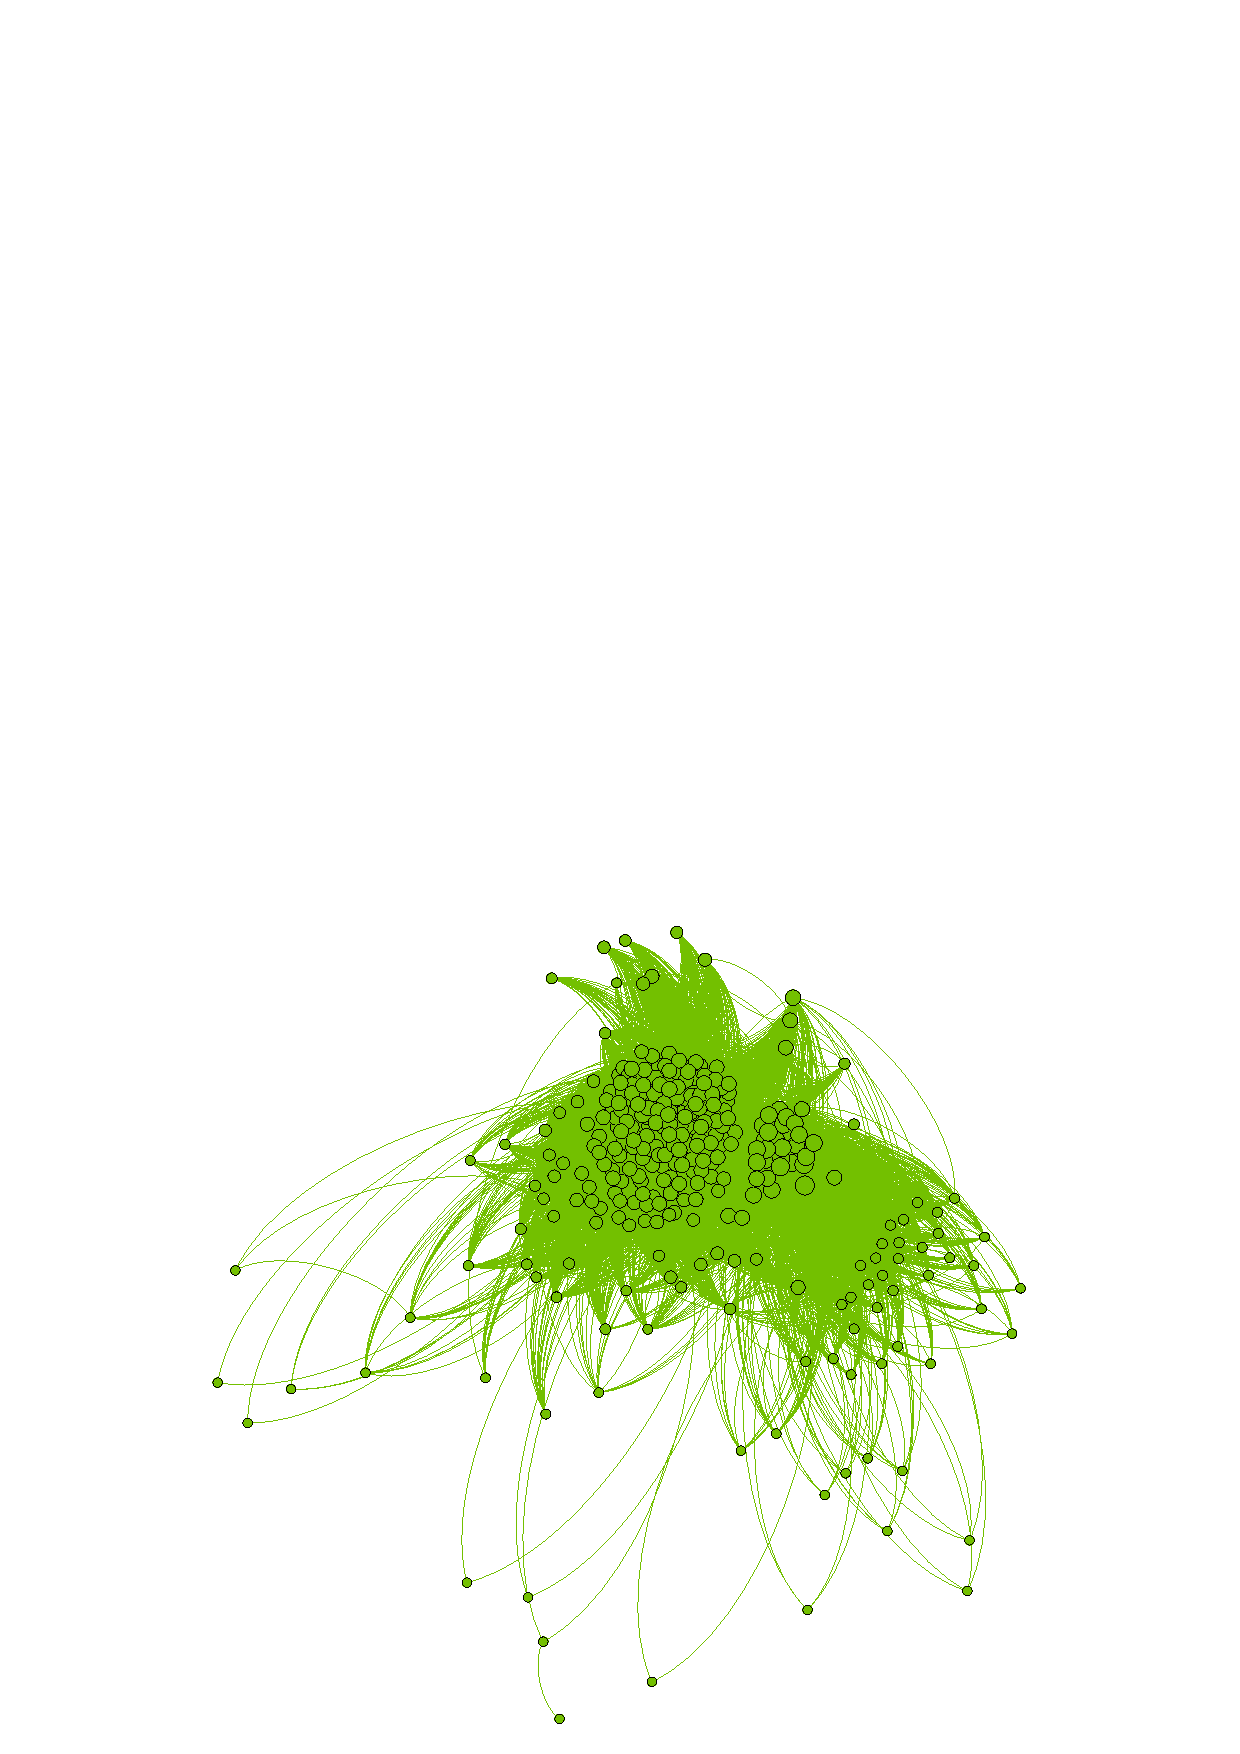
\includegraphics[width=0.45\textwidth]{community_2}%
		\label{fig:community_2}%
	}%
	\hfill%
	\subfloat[Livelihood]{%
		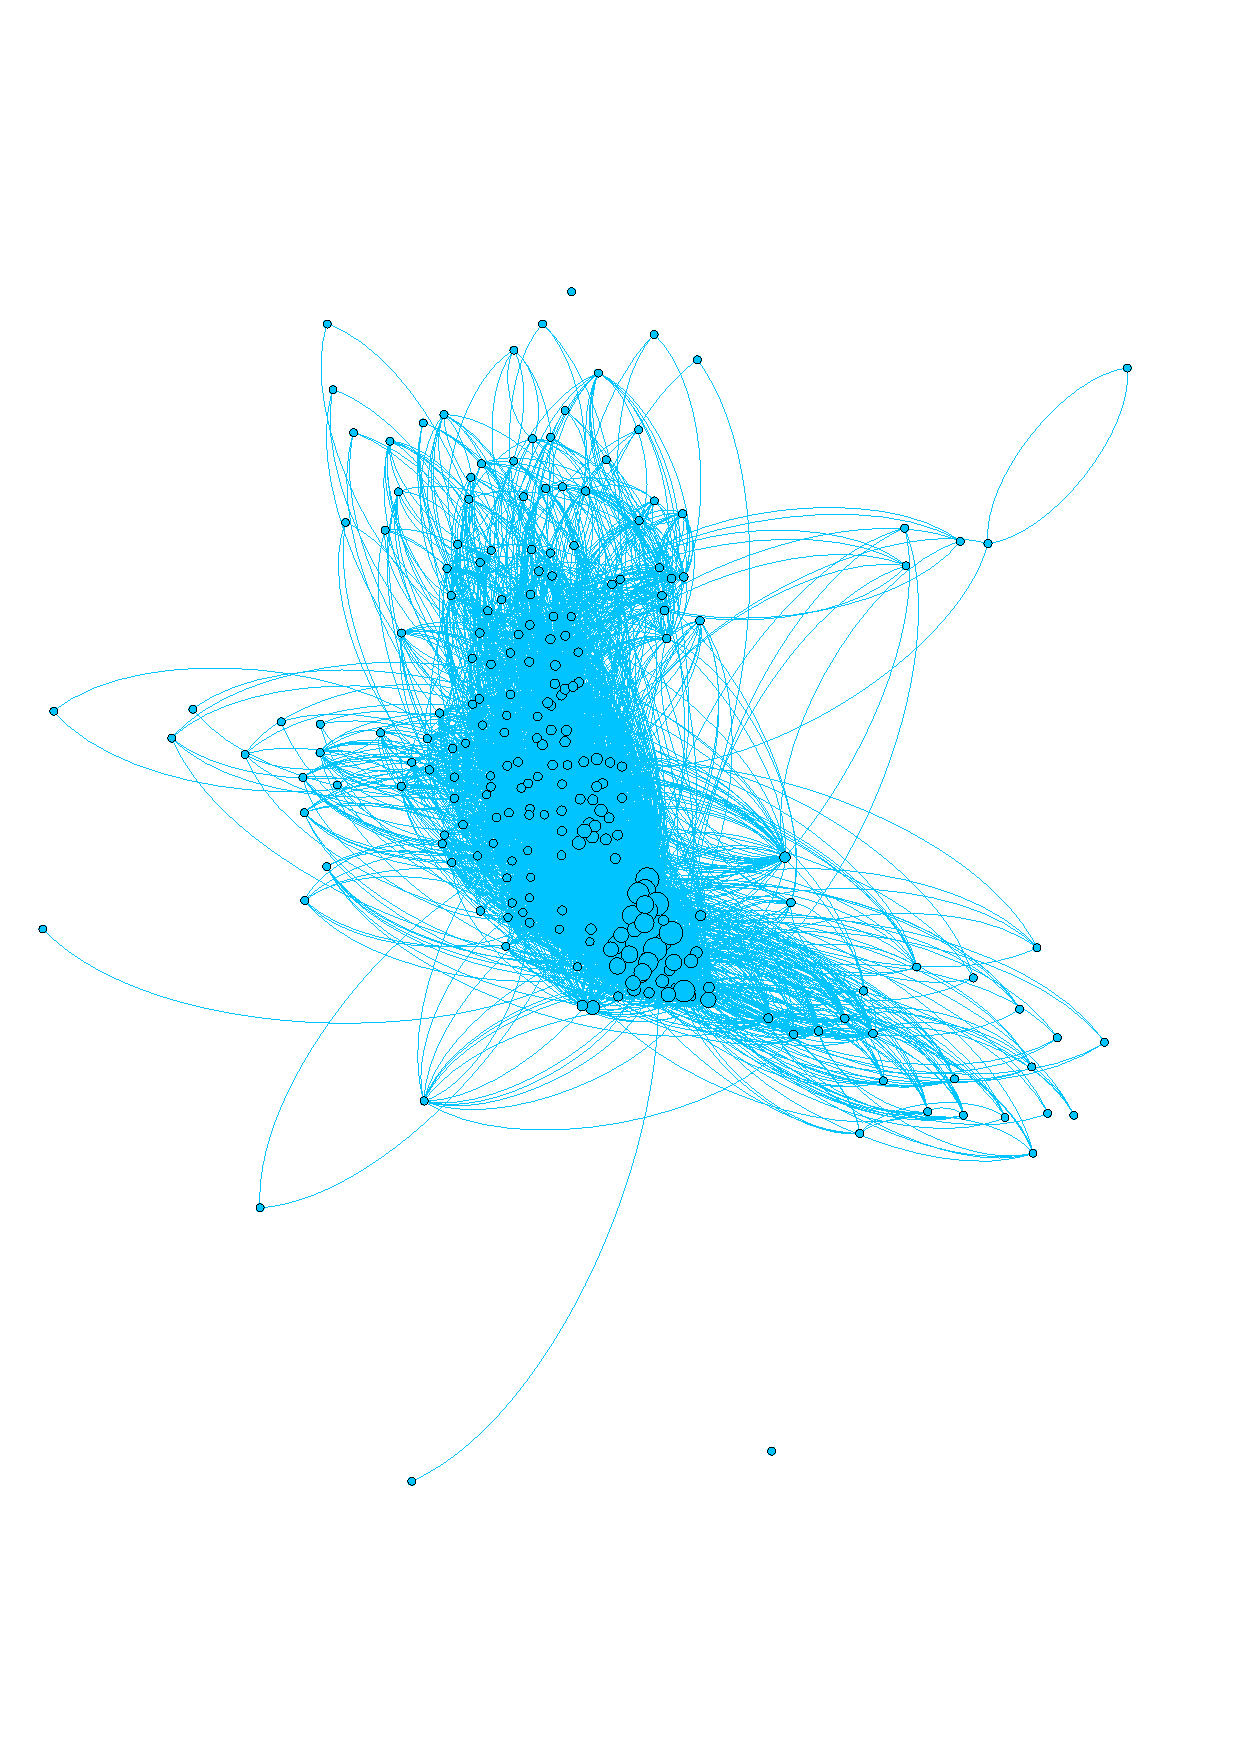
\includegraphics[width=0.45\textwidth]{community_3}%
		\label{fig:community_3}%
	}%
	\hfill%
	\subfloat[Insurance and chemical products]{%
		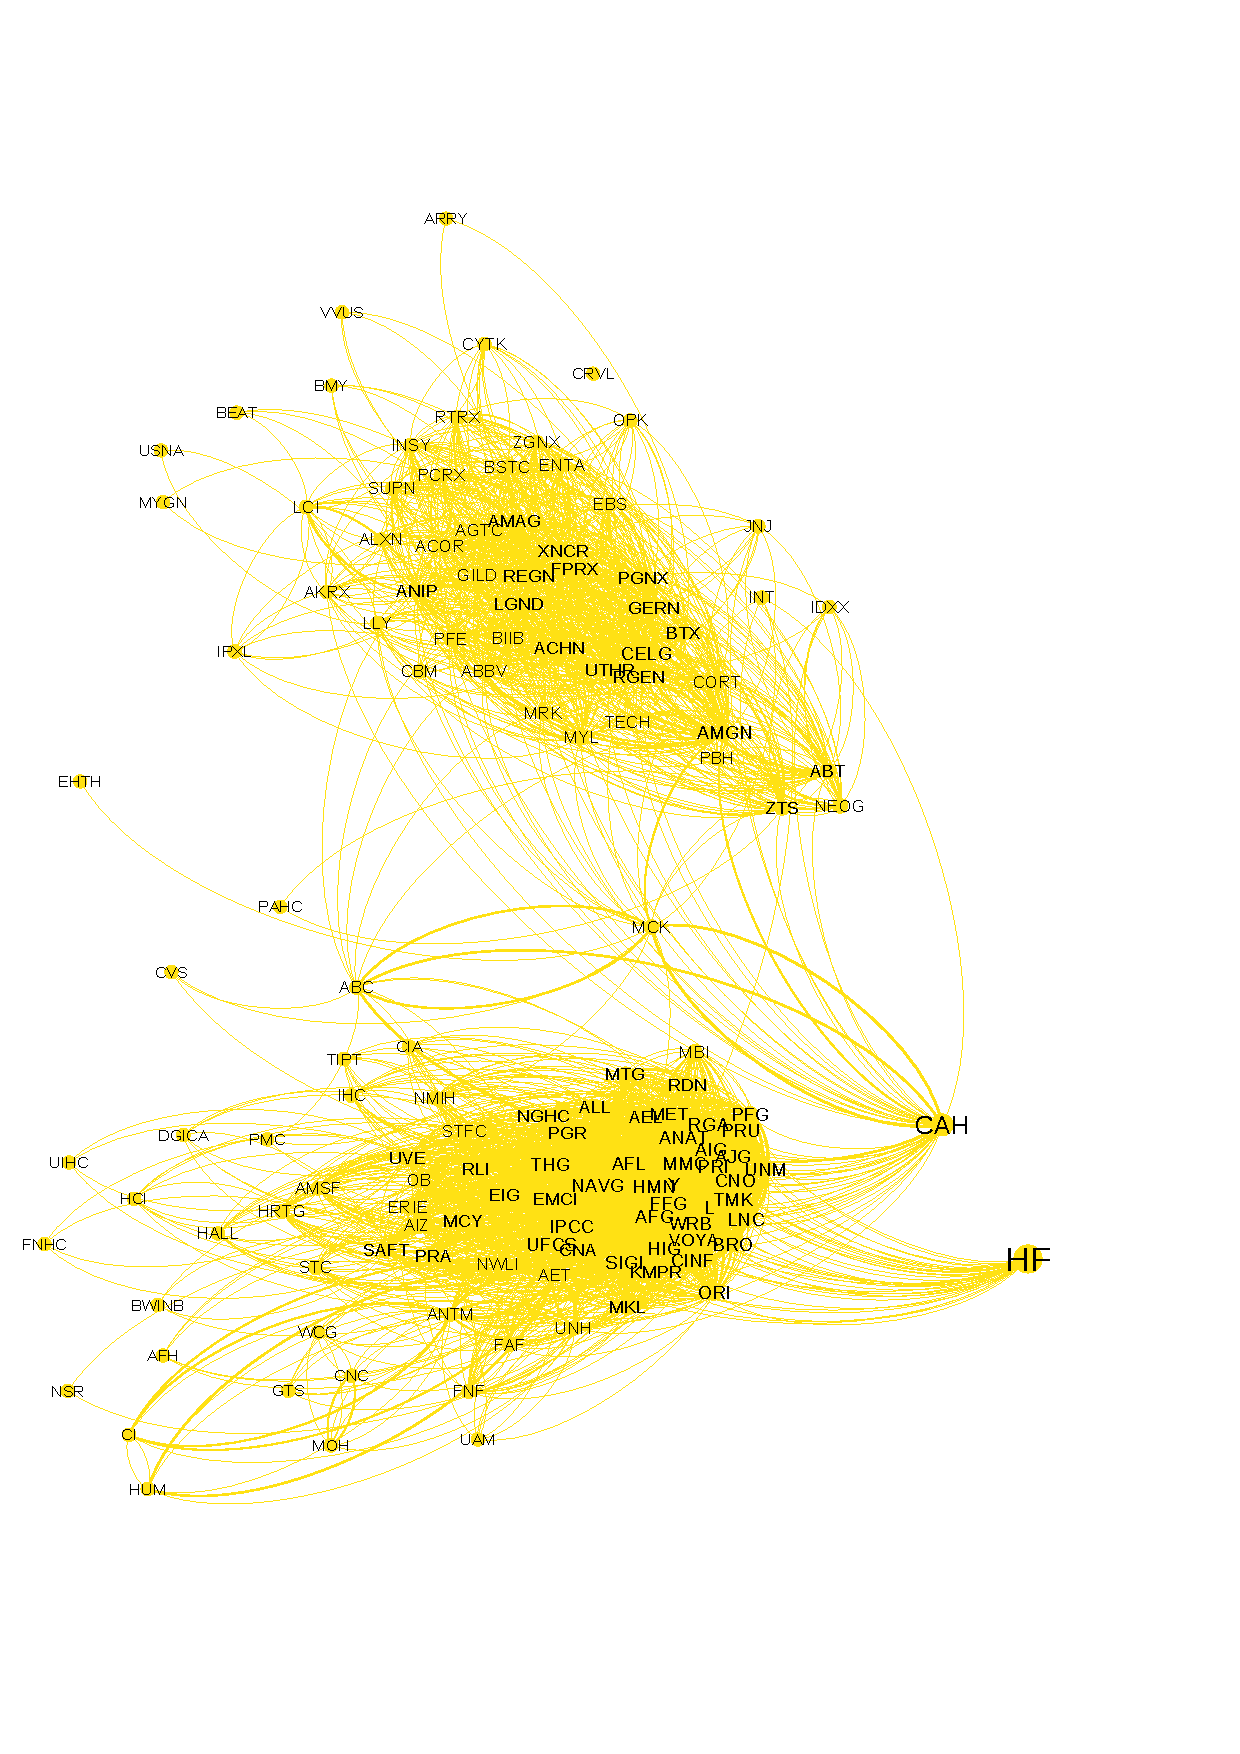
\includegraphics[width=0.45\textwidth]{community_4}%
		\label{fig:community_4}%
	}%
	\hfill%
	\subfloat[Utilities and financial vehicles]{%
		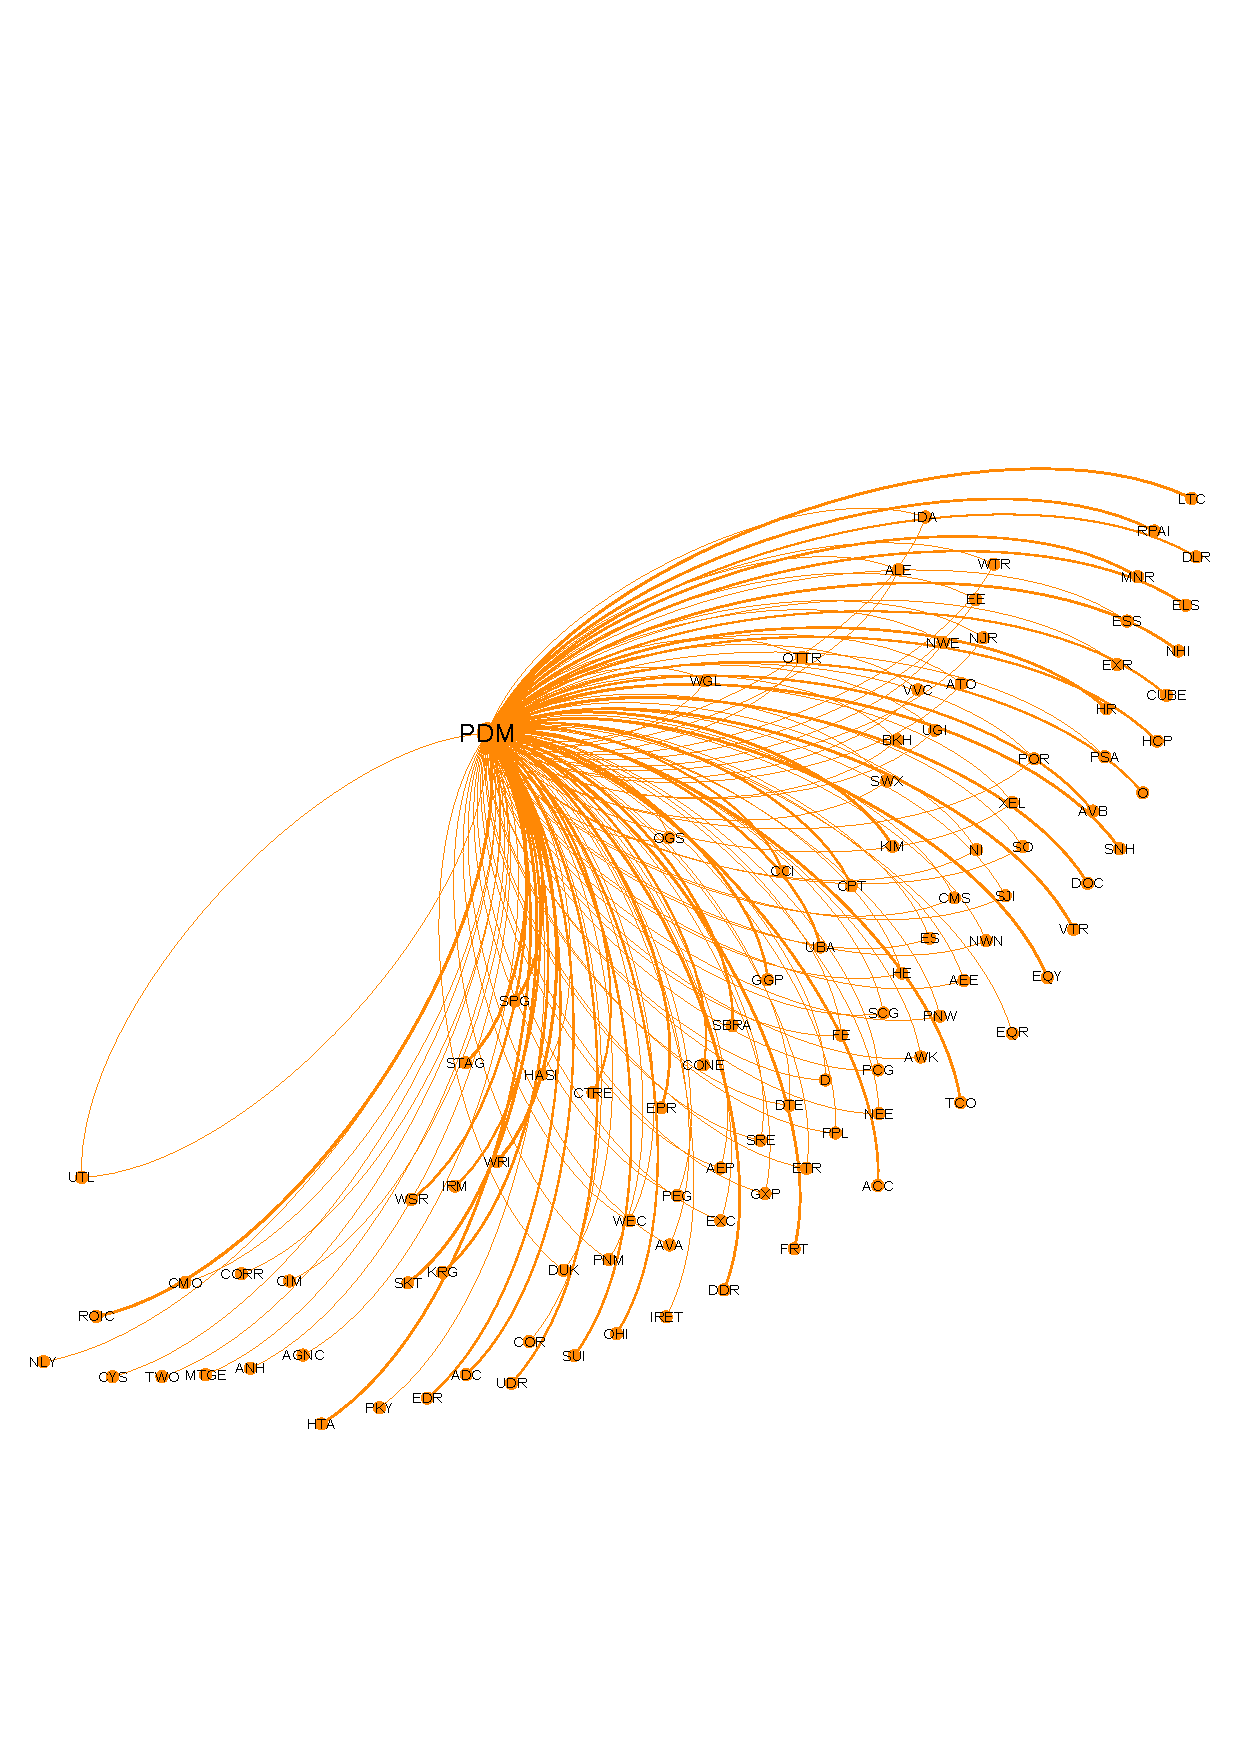
\includegraphics[width=0.45\textwidth]{community_5}%
		\label{fig:community_5}%
	}%
	\caption{Community sole views of the directed stock network. Stock tickers are displayed for the sparsely distributed communities.} \label{fig:distinctcommunities}
\end{figure}

\begin{figure} % 群落的行业柱形图
	\begin{center}
		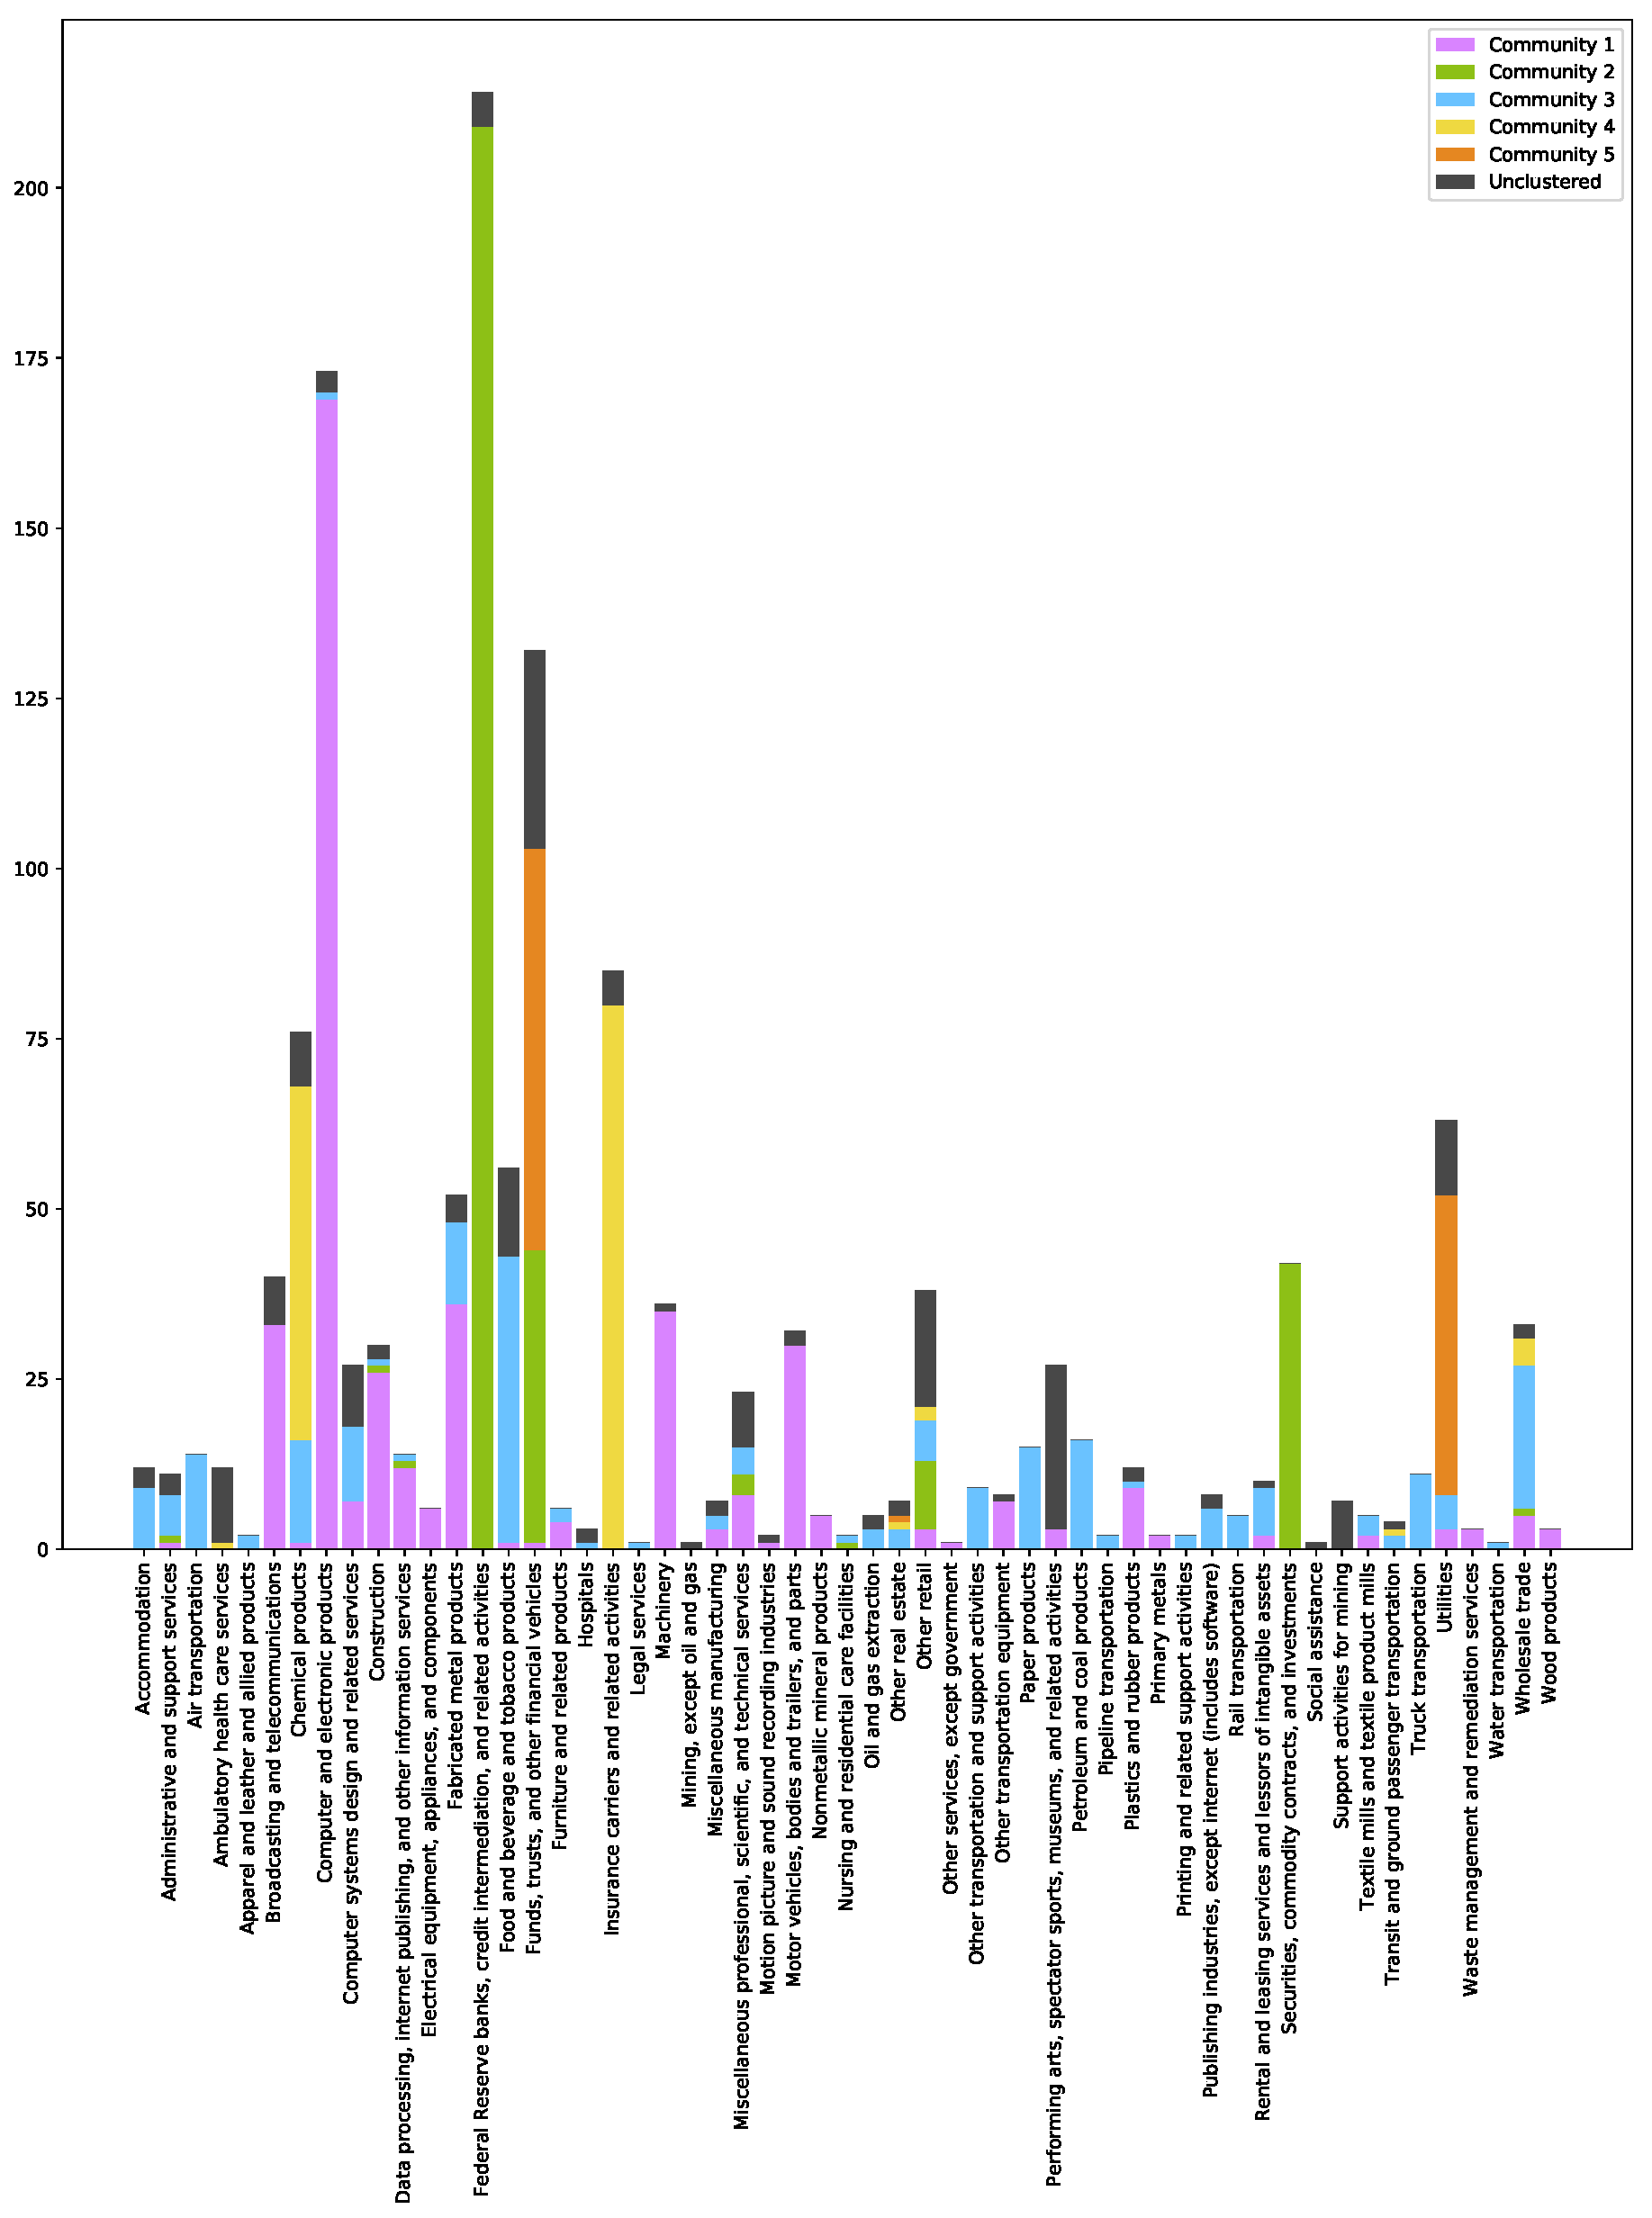
\includegraphics[width=15cm]{community_sector_stacked}
	\end{center}
	\caption{Stacked bar chart about the distribution of communities upon industrial sectors. Colours of stacks correspond to the colours of communities in figure~\ref{fig:community_graph} and figure~\ref{fig:distinctcommunities}, except the black stack indicating the nodes not belong to any communities. Sectors are arranged alphabetically.}
	\label{fig:community_sector_stacked}
\end{figure}

\begin{table}
	\begin{center}
		\begin{tabular}{|r|c|}\hline\hline
			&Undirected stock network\\\hline
			Degree distribution&Power-law\\
			Average out-degrees&Power-law\\
			Average path length&2.775\\
			Clustering coefficient&0.4675\\
			Global efficiency&0.2563\\
			Local efficiency&0.6276\\
			Assortativity&0.02004\\
			\hline\hline
		\end{tabular}
	\end{center}
	\caption{Main topologies of conventional stock price network}\label{tab:conventional}
\end{table}

\begin{figure}
	\subfloat[Empirical out-degree distribution]{%
		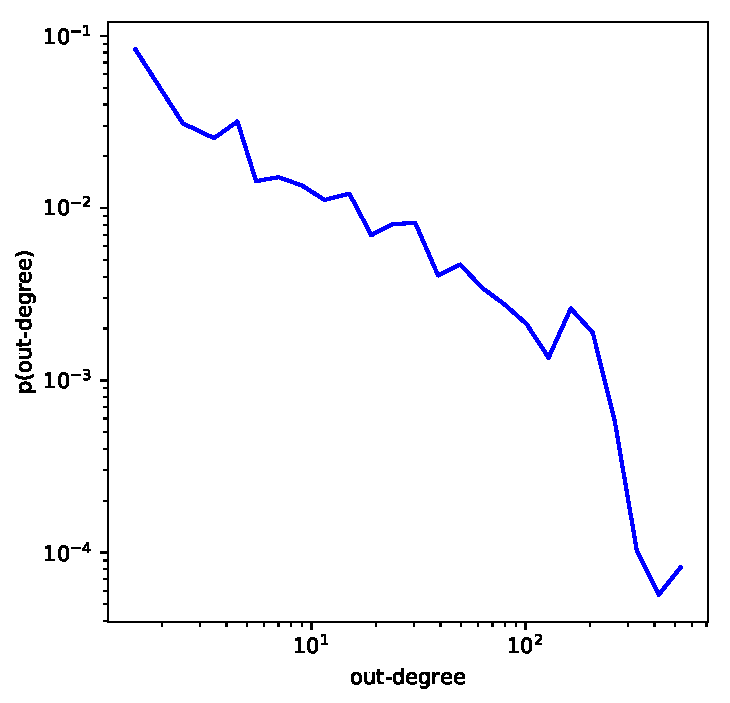
\includegraphics[width=0.46\textwidth]{G_out_degree_distribution_square}%
		\label{fig:G_out_degree_distribution_square}%
	}%
	\hfill%
	\subfloat[CCDF and power-law fit]{%
		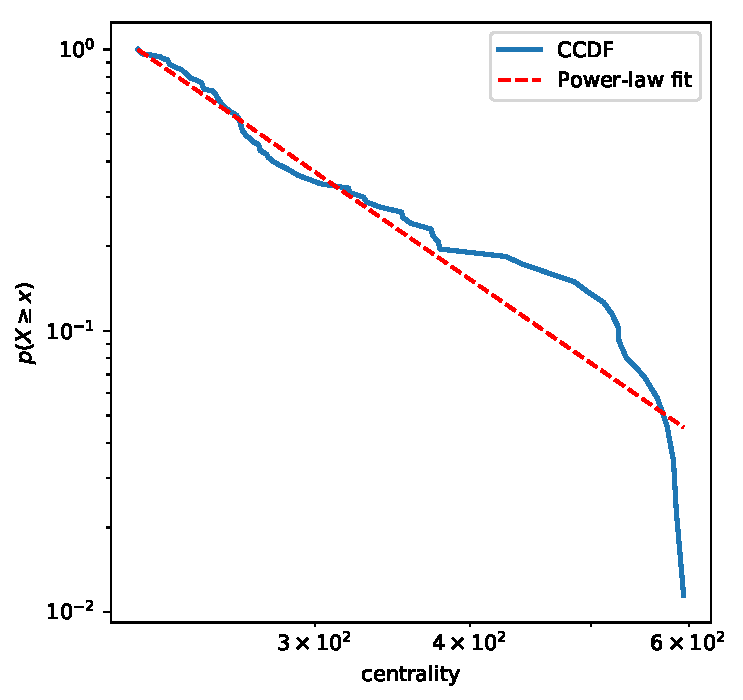
\includegraphics[width=0.465\textwidth]{out_degree_log_fit_square}%
		\label{fig:out_degree_log_fit_square}%
	}%
	\caption{Out-degree distribution of stock network} \label{fig:outdegreedistribution}
\end{figure}

\begin{figure} % P-P SW
	\centering
	\subfloat[Empirical out-degree distribution]{
		\label{subfig:G_sw_out_degree_distribution}
		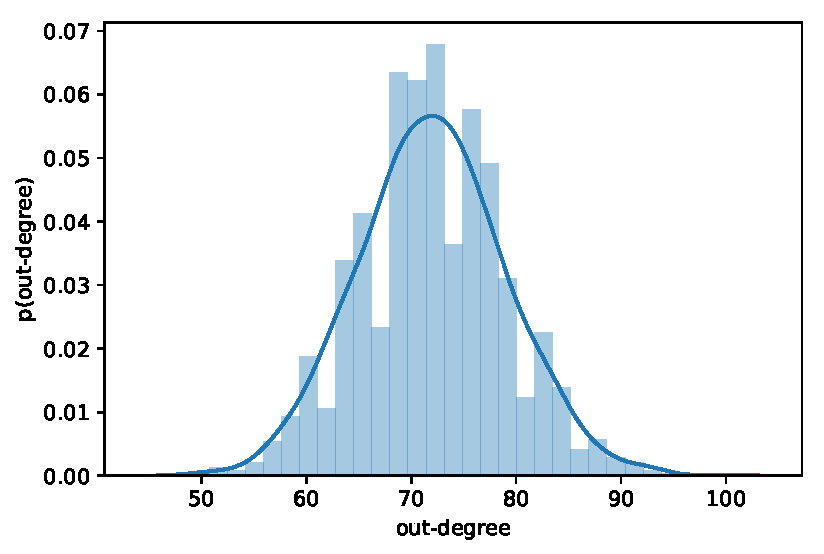
\includegraphics[width=12cm]{G_sw_out_degree_distribution} }
	
	\subfloat[P-P plot]{
		\label{subfig:G_ws_mat_prob_plot}
		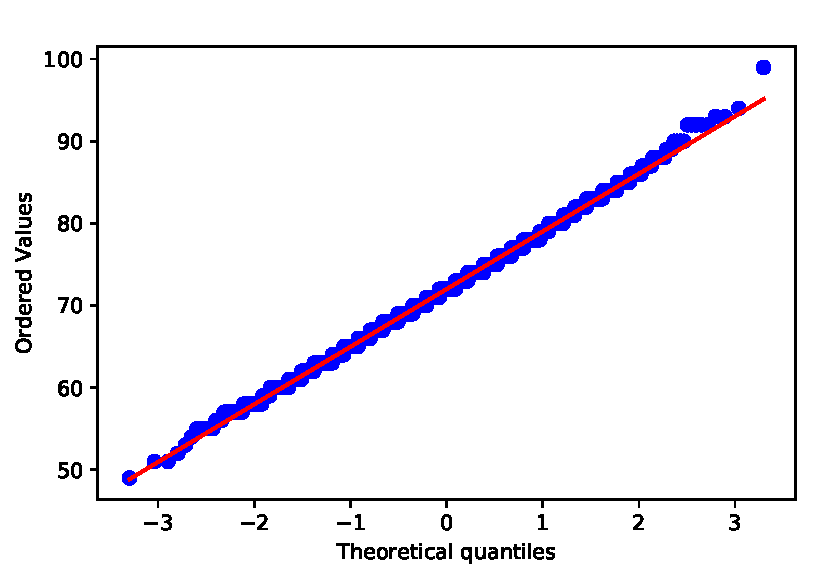
\includegraphics[width=12cm]{G_ws_mat_prob_plot} }
	
	\caption{Out-degree distribution and P-P plot of small-world network}
	\label{fig:distributionsm}
\end{figure}

\begin{figure} % P-P rd
	\centering
	\subfloat[Empirical out-degree distribution]{
		\label{subfig:G_rd_out_degree_distribution}
		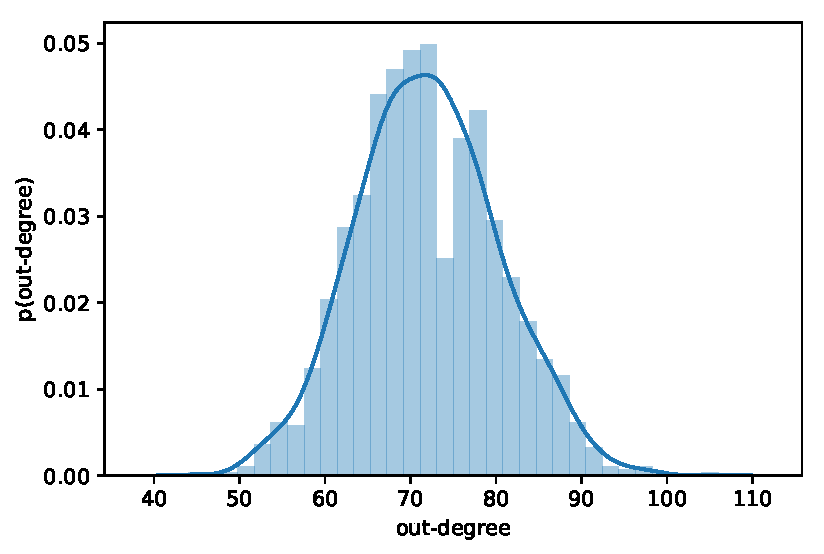
\includegraphics[width=12cm]{G_rd_out_degree_distribution} }
	
	\subfloat[P-P plot]{
		\label{subfig:G_rd_prob_plot}
		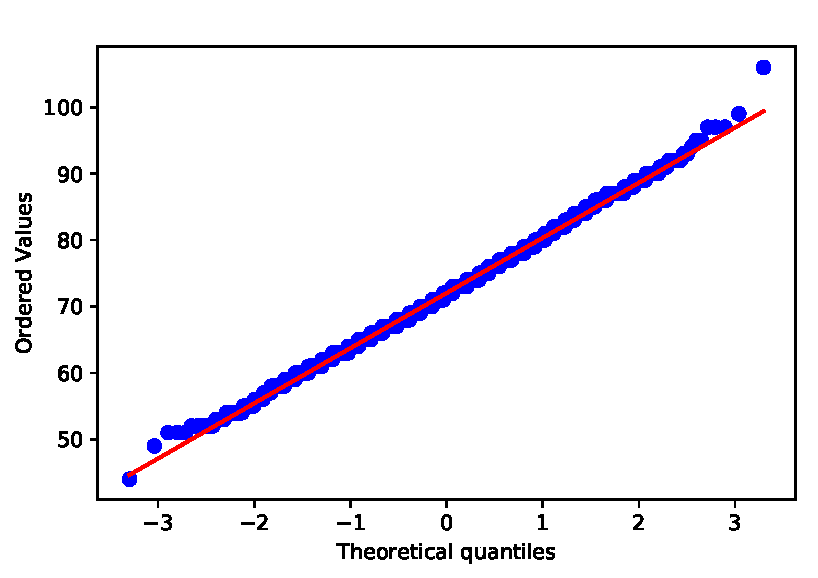
\includegraphics[width=12cm]{G_rd_prob_plot} }
	
	\caption{Out-degree distribution and P-P plot of random network}
	\label{fig:distributionrd}
\end{figure}


\iffalse
\begin{figure}
	\begin{center}
		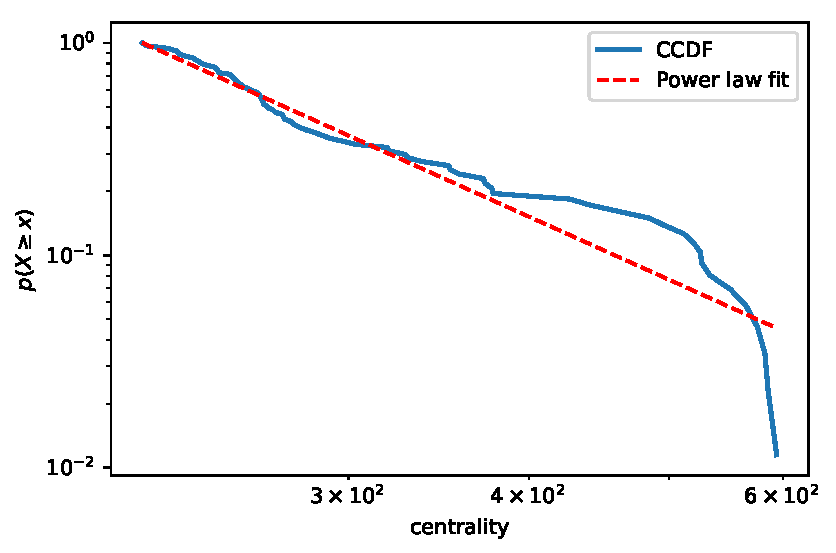
\includegraphics[width=15cm]{out_degree_log_fit}
	\end{center}
	\caption{Amounts of edges per EIO-threshold and correlation-coefficient-threshold}
	\label{fig:out_degree_log_fit}
\end{figure}
\fi

%Clustering coefficient
%行业内非对称边和行业间对称边的数量
%Global/ local efficiency

%Betweenness centrality


\section{Analysis of the directed weighted network}
\subsection{Topologies}

% Strength distribution
\begin{table}
	\begin{center}
		\begin{tabular}{|r|c|}\hline\hline
			&Weighted stock network\\\hline
			Strength distribution&Power-law\\
			Average strength&40.89\\ %40.88927702272619
			Average betweenness centrality&0.0007440\\
			Weighted assortativity&0.1244\\ % Assortativity with weight 0.12444731038165072
			\hline\hline
		\end{tabular}
	\end{center}
	\caption{Main topologies of weighted stock network}\label{tab:weighted}
\end{table}

\begin{figure}
	\subfloat[Bivariate distribution beween betweenness centralities of nodes and cumulative sums of stock daily return. The returns are actually logarithmic returns therefore the accumulation of all daily logarithmic returns in an entire year equals to a corresponding yearly logarithmic return.]{%
		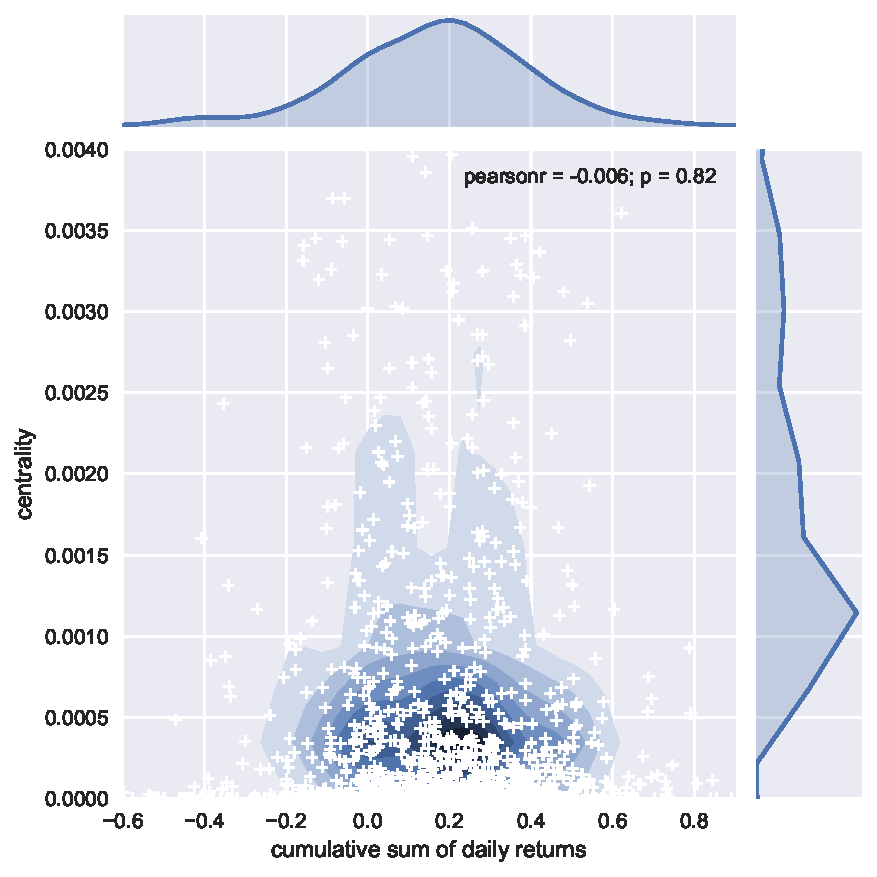
\includegraphics[width=0.46\textwidth]{sum_return_weighted_centrality}%
		\label{subfig:sum_return_weighted_centrality}%
	}%
	\hfill%
	\subfloat[Bivariate distribution beween betweenness centralities of nodes and standard deviations of stock daily return.]{%
		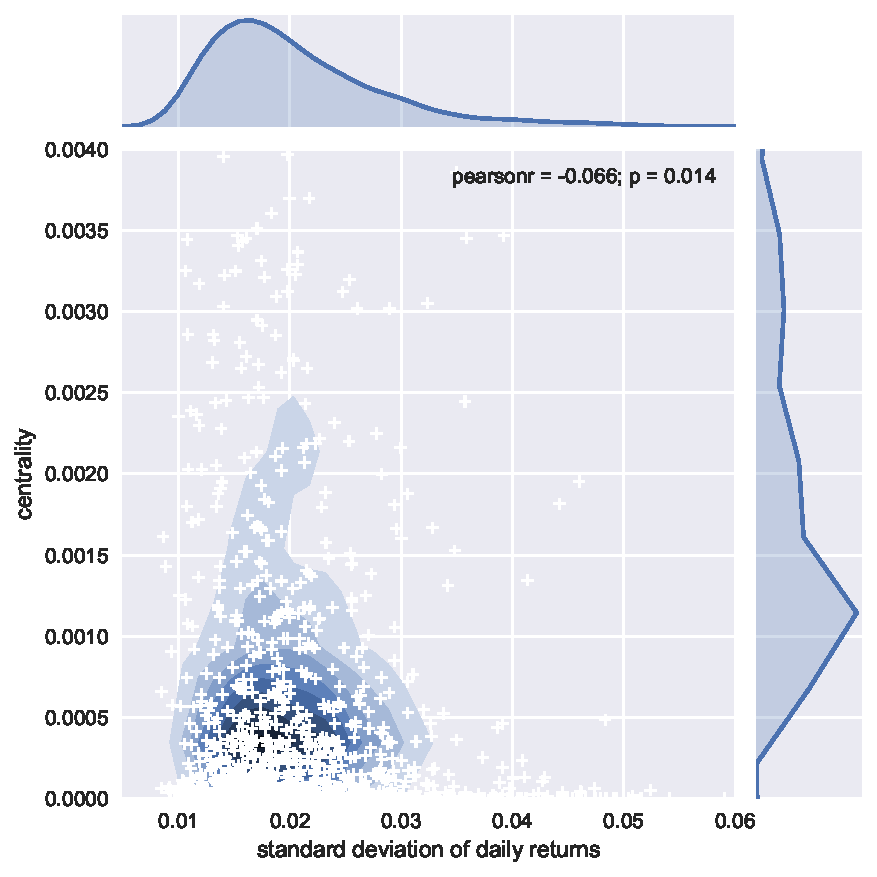
\includegraphics[width=0.465\textwidth]{std_return_weighted_centrality}%
		\label{subfig:std_return_weighted_centrality}%
	}%
	\caption{Bivariate distributions with betweenness centrality} \label{fig:bivariate}
\end{figure}

\subsection{Analysis on the relationship between price return and betweenness centrality}
Figures~\ref{fig:bivariate} reveal the relationships between betweenness centralities and price returns of stocks. First, in figure~\ref{subfig:sum_return_weighted_centrality} as much more nodes have low betweenness centrality values (lower than $0.001$), and the cumulative sum of returns fall intensively in the range of $(-0.1, 0.6)$, while that of the nodes with high betweenness centrality values (higher than $0.001$) also fall evenly in the same range Therefore, there is no significant difference between the expected return for stocks with different betweenness centrality values.

Second, according to the figure~\ref{subfig:std_return_weighted_centrality}, in spite of several outliers, as the betweenness centrality of nodes becomes higher, there will be a higher possibility of nodes tend to have low standard deviation of stock daily return. This indicates the hubs in the network have considerably stable return during the specified researched year among the whole stock market. The average standard deviation for all values of betweenness centrality remain similar because of the more frequent occurrences of outliers with higher betweenness centralities from the figure.

As a result, although choosing stocks with high centralities possibly will not bring a higher expected return for a portfolio, they have the functionality of decreasing the overall risks and generating more stable returns, which is also a vital feature for stock investment.


%\label{sec:community}
%\section{Stability of network}

%Industry

